\chapter{Example Applications} \label{chapter:interaction_techniques}
We have determined two levels of normal force at 2.7 kPa, and 3.375 kPa, referred to as light and strong forces, which are noticeable and discernible according to our studies of Absolute Detection Threshold (ADT) and Discrimination Threshold (JND). Based on FacePush, we introduce three VR applications embedded with the normal force haptic feedback on the face. In the first and second applications, the interaction provides discrete and continuous normal force depending on the duration of haptic feedback acting on a user's face. For the third, FacePush provides continuous normal force which are used to guide users toward a region of interest (ROI) when exploring 360 degree videos. 

\section{Boxing: Discrete Force on Face OK}

FacePush can provide discrete normal forces simulating immediate pressure acting on the face. This discrete haptic feedback was given a trial run in a virtual boxing scenario. Therein the user stays in a standing pose to experience our boxing application and the avatar of an opponent appears in front of the user in virtual reality.

As the application begins to run the play scenario, the opponent throws punches consecutively. As each punch hits the left, right, and middle of the user's virtual face, FacePush engages the left motor, right motor, and both motors, respectively. In addition to the area hit, distinguishable normal force stimuli are provided by FacePush that also simulate the varied strengths of the punches. (Figure \ref{fig:boxing}) displays examples of the force of the punches landed. The opponent is programmed to randomly throw jabs, straight blows or hooks from left or right. A jab is fast and light. A straight punch is a longer punch of a medium strength. A hook is a curvy punch with great strength. We mapped the strength of each punch onto the two levels of normal force provided by FacePush. The area hit and the strength of a punch are calculated in real time from the opponents boxing motions. 
%A health bar was displayed to remind the user of her/his remaining health points. 

An emoji is displayed on the lower-left area of the user's field of view (FOV) which area for where each hit is landed. Users experience different kinds of punches and they also suffer different degrees of virtual damage. At the moment of being hit, the camera view of the user shakes instantly as a visual stimulus, and the motors will rotate according to the strength and area hit simultaneously providing haptic feedback on the face.

\begin{figure}[h]
    \begin{center}
        \begin{tabular}{@{\hspace{0.1cm}}c}
            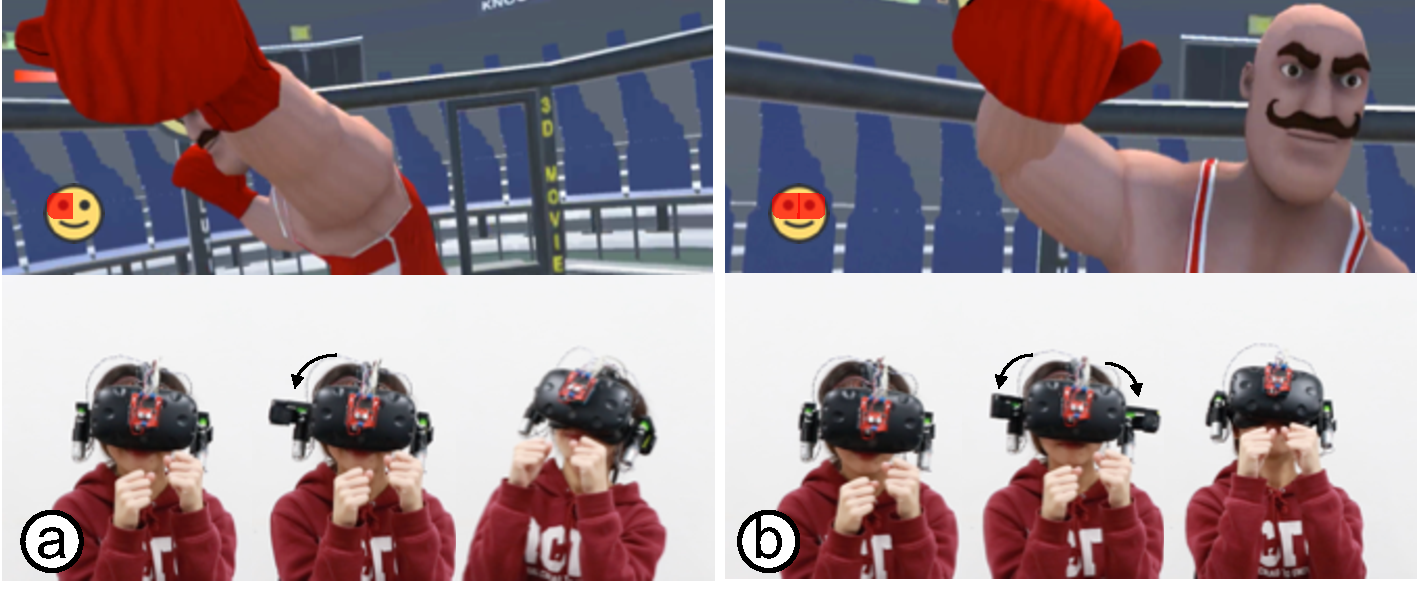
\includegraphics[width=1\linewidth]{figures/boxing2}
        \end{tabular}
        \caption{Boxing experience: a punch hit at the left and middle areas of the user face triggers the left and both motors respectively. (The mark on the cloth was masked for blind review.)}
        \label{fig:boxing}
    \end{center}
\end{figure}

\section{Diving: Continuous and Discrete Normal Force OK}

Continuous normal force simulates pressure acting on a face over a time span, e.g., the flow of water acting on the face when swimming creates a continuous pressure on the face. In this virtual experience, we created a diving scenario to demonstrate the haptic feedback of the pressure of water flowing across the face. 

The user is seated in a chair and wears wrist straps on both forearms each attached to a Vive tracker. The Vive trackers record the orbits of the hands' positions. When a user makes actions with the hand similar to say a breaststroke for example, the orbits of the two trackers are used to calculate the direction of motion and speed of the user virtually. A left-arm stroke leads to a right turn and a right-arm stroke leads to a left turn. If the user makes arm strokes with both hands, she/he will move forward (Figure \ref{fig:diving-fishshark}(a-b)). Meanwhile, a corresponding normal force is generated to simulate the water flowing across the face. For example, while swimming to the right, the right motor will give force to the right side of the user's face. If the user is moving forward, both motors start turning to a specific angle and keep holding the belt during the advancing term. Depending on the speeds of motion, we set the force to increase up to light or medium level and then fade out the force.

In the diving scenario, we also present two underwater haptic experiences, as displayed in (Figure \ref{fig:diving-fishshark}(c-d)). Users can experience passing through a school of fish.
A user's face will receive a normal force alternating on their left and right sides. FacePush simulates the experience with light force. In the second experience, a shark swims toward the user and then turns away at close range; the current from this virtual encounter exerts a strong normal force on the user's face.

\begin{figure}[h]
    \begin{center}
        \begin{tabular}{@{\hspace{0.1cm}}c}
            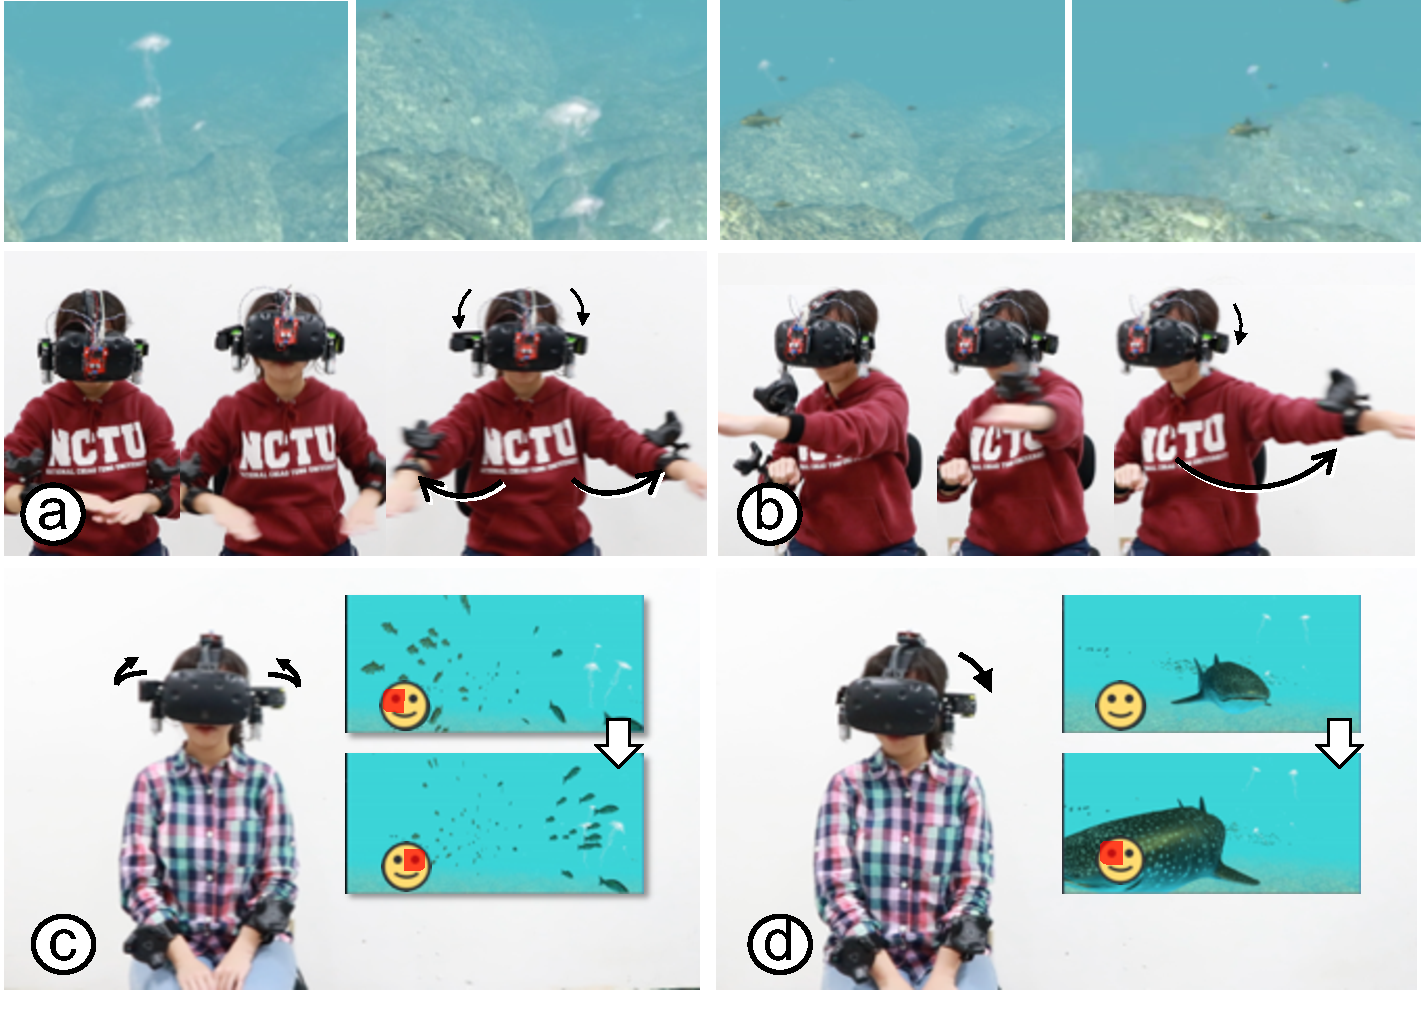
\includegraphics[width=1\linewidth]{figures/diving-fishshark2}
        \end{tabular}
        \caption{Diving experience: the user advances underwater with arm strokes of both hands, and turn left with right-arm strokes.  (The mark on the cloth was masked for blind review.)}
        \label{fig:diving-fishshark}
    \end{center}
\end{figure}

\section{Attention Guidance: Continuous Normal Force OK}

The users of 360 degree videos sometime suffer from missing regions of interests (ROI) in any given video clip. In this implementation of FacePush, we mapped the normal forces generated by the left and right torque generators onto a directional cue of yaw axis in 360 degree videos. 

%Lin et al. \cite{} proposed using a picture-in-picture technique and show which side should the user rotate to 
Here, the normal force generated by FacePush exerted on the user's face is used to prompt targets for the attention of the viewer in 360 degree videos. That is, when a target is beyond the user's field of view on the left side of the user, FacePush engages the left motor to indicate the target's direction. The intensity of normal force is determined based on the rotational angle to bring the target into the FOV. When the angle is less than 30 degrees, a light force is applied; otherwise, a medium force is applied. Once the target appears in the user's field of view (FOV), the force disappears. This trial implementation utilizes a sample wildlife 360 degree video (Figure \ref{fig:attention-guidance}). The user looks for animals on a plain, and FacePush prompts the user to locate where there the animals are.

\begin{figure}[h]
    \begin{center}
        \begin{tabular}{@{\hspace{0.1cm}}c}
            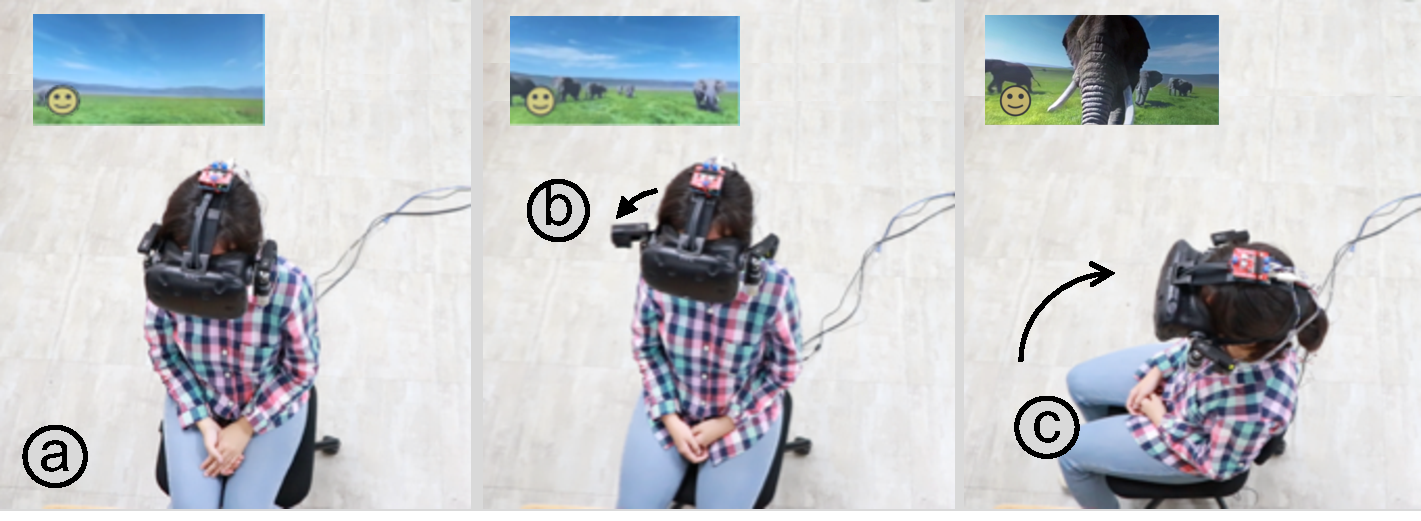
\includegraphics[width=1\linewidth]{figures/attention-guidance2}
        \end{tabular}
        \caption{Attention Guidance: left or right-sided normal force on face guides users to search toward left or right respectively.}
        \label{fig:attention-guidance}
    \end{center}
\end{figure}